This supplement documents data, measures, measurement-comparability tests, the full multilevel results, robustness checks, and a descriptive longitudinal panel. Section numbers are referenced from the main text. All analyses use ISSP 2023 (ZA10010 v1.0.0); country-level moderators use V-Dem v15 (2023 values).

\section{SI-A. Measures and coding}\label{si-a.-measures-and-coding}

All items are rescaled to \([0,1]\) and oriented so higher = more of the named concept. ISSP \texttt{WEIGHT\_COM} (combined weight) is used for the descriptive and reliability estimates, normalized for pooled estimates so each country contributes equally; the multilevel models in the main text are unweighted, with design-weighted versions reported as a robustness check (SI-J). Item codings were verified against the ZA10010 value labels.

{\small\begin{longtable}[]{@{}
  >{\raggedright\arraybackslash}p{(\linewidth - 4\tabcolsep) * \real{0.3333}}
  >{\raggedright\arraybackslash}p{(\linewidth - 4\tabcolsep) * \real{0.3333}}
  >{\raggedright\arraybackslash}p{(\linewidth - 4\tabcolsep) * \real{0.3333}}@{}}
\toprule\noalign{}
\begin{minipage}[b]{\linewidth}\raggedright
Construct
\end{minipage} & \begin{minipage}[b]{\linewidth}\raggedright
ISSP items (2023)
\end{minipage} & \begin{minipage}[b]{\linewidth}\raggedright
Scaling
\end{minipage} \\
\midrule\noalign{}
\endhead
\bottomrule\noalign{}
\figcap{Constructs, ISSP 2023 items, and scaling}{All items rescaled to $[0,1]$, oriented so higher means more of the named concept.}\\
\endlastfoot
Democratic rights (principles) & v42 minority rights, v43 participation, v44 civil disobedience (``how important \emph{for democracy}'', 1--7) & \((x-1)/6\); higher = more important \\
Democratic performance & v38 ``how well does democracy work in {[}country{]} today'' (0--10) & \(x/10\); higher = works well \\
Ascriptive membership & v1 born, v3 religion, v6 ancestry (1--4 importance); v13 born-not-effort & reverse to higher = more ascriptive \\
Civic membership & v2 citizenship, v4 respect institutions, v5 feel national & higher = more important \\
National superiority & v9 world better if like us, v10 better than most, v11 support when wrong (1--5 agree) & higher = more agreement \\
Anti-immigrant exclusion & v26 crime, v27 economy (rev.), v28 jobs, v29 ideas (rev.), v30 native preference, v31 reduce number & higher = more exclusionary \\
Protectionism & v20--v25 (imports, sovereignty, foreign land, etc.) & higher = more protectionist \\
National pride & v15--v19 (political influence, economy, sports, arts, history); pride in democracy (v14) excluded & higher = prouder \\
\end{longtable}}

Individual controls: age (years), gender (female = 1), education (ISCED 0--8), left--right self-placement (v46, 0--10, rescaled to the unit interval). The democratic-rights battery (v41--v44) is unique to the 2023 module; earlier ISSP National Identity rounds (1995/2003/2013) do not field it, which is why the relational analysis is cross-sectional (see SI-K).

The four-item democratic-rights index (adding v41, ``adequate standard of living'') mixes liberal rights with welfare commitments; the three-item liberal-rights index is used in the main analysis. Results are unchanged with the four-item version.

\clearpage
\section{SI-B. Countries, V-Dem indices, and the content of nationhood}\label{si-b.-countries-v-dem-indices-and-the-content-of-nationhood}

29 countries, \(N = 43{,}517\). Countries are ordered by the civic--ethnic content of nationhood (country-mean ascriptive membership), the main moderator. Note that East Asian democracies (Taiwan, South Korea) score high on V-Dem's liberal component yet have markedly more ascriptive conceptions of nationhood than the Western core.

{\small\begin{longtable}[]{@{}
  >{\raggedright\arraybackslash}p{(\linewidth - 12\tabcolsep) * \real{0.1400}}
  >{\raggedright\arraybackslash}p{(\linewidth - 12\tabcolsep) * \real{0.1750}}
  >{\raggedright\arraybackslash}p{(\linewidth - 12\tabcolsep) * \real{0.1500}}
  >{\raggedleft\arraybackslash}p{(\linewidth - 12\tabcolsep) * \real{0.1300}}
  >{\raggedleft\arraybackslash}p{(\linewidth - 12\tabcolsep) * \real{0.1300}}
  >{\raggedleft\arraybackslash}p{(\linewidth - 12\tabcolsep) * \real{0.1350}}
  >{\raggedleft\arraybackslash}p{(\linewidth - 12\tabcolsep) * \real{0.1000}}@{}}
\toprule\noalign{}
\begin{minipage}[b]{\linewidth}\raggedright
Country
\end{minipage} & \begin{minipage}[b]{\linewidth}\raggedright
Region-regime group
\end{minipage} & \begin{minipage}[b]{\linewidth}\raggedright
V-Dem RoW 2023
\end{minipage} & \begin{minipage}[b]{\linewidth}\raggedleft
Liberal comp.
\end{minipage} & \begin{minipage}[b]{\linewidth}\raggedleft
Electoral comp.
\end{minipage} & \begin{minipage}[b]{\linewidth}\raggedleft
Mean ascriptive
\end{minipage} & \begin{minipage}[b]{\linewidth}\raggedleft
\(N\)
\end{minipage} \\
\midrule\noalign{}
\endhead
\bottomrule\noalign{}
\figcap{Countries, V-Dem indices, and the content of nationhood}{Ordered by the civic--ethnic content of nationhood (country-mean ascriptive membership). East Asian democracies (Taiwan, South Korea) score high on the liberal component yet are markedly more ascriptive.}\\
\endlastfoot
Canada & Western dem. & Electoral dem. & 0.88 & 0.85 & 0.24 & 2,127 \\
Sweden & Western dem. & Liberal dem. & 0.98 & 0.88 & 0.25 & 1,607 \\
Australia & Western dem. & Liberal dem. & 0.96 & 0.85 & 0.28 & 993 \\
New Zealand & Western dem. & Liberal dem. & 0.95 & 0.88 & 0.32 & 1,191 \\
Norway & Western dem. & Liberal dem. & 0.95 & 0.88 & 0.33 & 1,132 \\
Finland & Western dem. & Liberal dem. & 0.97 & 0.86 & 0.35 & 1,369 \\
Denmark & Western dem. & Liberal dem. & 0.98 & 0.92 & 0.35 & 1,254 \\
Switzerland & Western dem. & Liberal dem. & 0.96 & 0.89 & 0.36 & 3,202 \\
Germany & Western dem. & Liberal dem. & 0.97 & 0.85 & 0.36 & 1,545 \\
United States & Western dem. & Liberal dem. & 0.92 & 0.84 & 0.36 & 1,589 \\
Netherlands & Western dem. & Liberal dem. & 0.95 & 0.84 & 0.36 & 1,509 \\
France & Western dem. & Liberal dem. & 0.93 & 0.88 & 0.37 & 1,905 \\
Slovenia & E. Europe dem. & Electoral dem. & 0.87 & 0.76 & 0.40 & 1,039 \\
Austria & Western dem. & Electoral dem. & 0.93 & 0.85 & 0.41 & 1,146 \\
Taiwan & E. Asian dem. & Liberal dem. & 0.88 & 0.82 & 0.42 & 1,563 \\
Greece & Western dem. & Electoral dem. & 0.77 & 0.74 & 0.45 & 1,463 \\
Israel & Other dem. & Electoral dem. & 0.89 & 0.72 & 0.48 & 1,197 \\
Italy & Western dem. & Liberal dem. & 0.91 & 0.82 & 0.55 & 1,135 \\
South Korea & E. Asian dem. & Liberal dem. & 0.87 & 0.73 & 0.58 & 1,230 \\
Mexico & Other dem. & Electoral dem. & 0.47 & 0.55 & 0.60 & 1,025 \\
Lithuania & E. Europe dem. & Electoral dem. & 0.94 & 0.79 & 0.60 & 1,257 \\
Hungary & E. Europe non-dem. & Electoral autoc. & 0.66 & 0.44 & 0.61 & 1,023 \\
Croatia & E. Europe dem. & Electoral dem. & 0.88 & 0.74 & 0.61 & 1,400 \\
Slovakia & E. Europe dem. & Electoral dem. & 0.90 & 0.82 & 0.61 & 1,025 \\
India & S/SE Asia non-dem. & Electoral autoc. & 0.62 & 0.37 & 0.64 & 1,605 \\
Russia & E. Europe non-dem. & Electoral autoc. & 0.15 & 0.19 & 0.65 & 1,574 \\
Thailand & S/SE Asia non-dem. & Electoral autoc. & 0.64 & 0.29 & 0.67 & 1,500 \\
South Africa & Other dem. & Electoral dem. & 0.86 & 0.70 & 0.73 & 3,112 \\
Philippines & S/SE Asia non-dem. & Electoral autoc. & 0.60 & 0.43 & 0.79 & 1,800 \\
\end{longtable}}

The simple regime binary used for robustness (SI-J) codes V-Dem liberal and electoral democracies as democracies and electoral/closed autocracies as non-democracies, yielding 24 democracies and 5 non-democracies (Hungary, India, Philippines, Russia, Thailand).

\clearpage
\section{SI-C. Scale reliability by region-regime group}\label{si-c.-scale-reliability-by-region-regime-group}

Cronbach's \(\alpha\) (unweighted). The democratic-rights index is modest in the West (\(\alpha = 0.50\)) and stronger elsewhere; the anti-immigrant index is strong in Western and East European democracies but weak in South/Southeast Asia, foreshadowing the non-invariance documented in SI-D.

{\small\begin{longtable}[]{@{}
  >{\raggedright\arraybackslash}p{(\linewidth - 10\tabcolsep) * \real{0.1304}}
  >{\raggedleft\arraybackslash}p{(\linewidth - 10\tabcolsep) * \real{0.1739}}
  >{\raggedleft\arraybackslash}p{(\linewidth - 10\tabcolsep) * \real{0.1739}}
  >{\raggedleft\arraybackslash}p{(\linewidth - 10\tabcolsep) * \real{0.1739}}
  >{\raggedleft\arraybackslash}p{(\linewidth - 10\tabcolsep) * \real{0.1739}}
  >{\raggedleft\arraybackslash}p{(\linewidth - 10\tabcolsep) * \real{0.1739}}@{}}
\toprule\noalign{}
\begin{minipage}[b]{\linewidth}\raggedright
Group
\end{minipage} & \begin{minipage}[b]{\linewidth}\raggedleft
Dem. rights
\end{minipage} & \begin{minipage}[b]{\linewidth}\raggedleft
Ascriptive
\end{minipage} & \begin{minipage}[b]{\linewidth}\raggedleft
Superiority
\end{minipage} & \begin{minipage}[b]{\linewidth}\raggedleft
Anti-immigrant
\end{minipage} & \begin{minipage}[b]{\linewidth}\raggedleft
Pride
\end{minipage} \\
\midrule\noalign{}
\endhead
\bottomrule\noalign{}
\figcap{Scale reliability (Cronbach's $\alpha$) by region-regime group}{Unweighted Cronbach's $\alpha$. The anti-immigrant index is weak in South/Southeast Asia, foreshadowing SI-D.}\\
\endlastfoot
Western democracies & 0.50 & 0.75 & 0.59 & 0.86 & 0.66 \\
Eastern Europe democracies & 0.77 & 0.68 & 0.73 & 0.79 & 0.70 \\
Eastern Europe non-democracies & 0.63 & 0.64 & 0.80 & 0.74 & 0.83 \\
East Asian democracies & 0.57 & 0.71 & 0.46 & 0.65 & 0.67 \\
South/SE Asia non-democracies & 0.70 & 0.49 & 0.62 & 0.37 & 0.74 \\
Other democracies & 0.67 & 0.56 & 0.61 & 0.67 & 0.74 \\
\end{longtable}}

\clearpage
\section{SI-D. Measurement invariance}\label{si-d.-measurement-invariance}

The analysis compares \emph{associations} across contexts, not scale means, and the invariance tests justify exactly that restriction. A multi-group confirmatory factor analysis across the six region-regime groups (ML, with FIML for missingness) tests configural, metric, and scalar invariance, using the decision rule \(\Delta\text{CFI} \geq -0.010\) \citep{cheung2002goodness}.

{\small\begin{longtable}[]{@{}llrrrr@{}}
\toprule\noalign{}
Scale & Level & CFI & RMSEA & SRMR & \(\Delta\)CFI \\
\midrule\noalign{}
\endhead
\bottomrule\noalign{}
\figcap{Multi-group measurement invariance across the six region-regime groups}{Metric invariance permits comparison of associations; scalar invariance, required to compare scale \emph{means}, is decisively rejected for every scale ($\Delta$CFI from $-0.11$ to $-0.23$).}\\
\endlastfoot
Anti-immigrant (6) & configural & 0.904 & 0.133 & 0.052 & --- \\
& metric & 0.880 & 0.123 & 0.065 & −0.024 \\
& scalar & 0.722 & 0.163 & 0.119 & −0.158 \\
Ascriptive (4) & configural & 0.993 & 0.054 & 0.015 & --- \\
& metric & 0.981 & 0.060 & 0.035 & −0.012 \\
& scalar & 0.874 & 0.122 & 0.093 & −0.107 \\
Superiority (3) & configural & 1.000 & 0.000 & 0.000 & --- \\
& metric & 0.968 & 0.091 & 0.042 & −0.032 \\
& scalar & 0.775 & 0.172 & 0.090 & −0.193 \\
Democratic rights (3) & configural & 1.000 & 0.000 & 0.000 & --- \\
& metric & 0.977 & 0.072 & 0.032 & −0.023 \\
& scalar & 0.747 & 0.168 & 0.091 & −0.230 \\
\end{longtable}}

Configural invariance holds. Metric invariance is only approximate. The loading-equality fit change runs from −0.012 to −0.032, modestly beyond the conventional −0.010 guideline for all four scales, but an order of magnitude smaller than the scalar change. Scalar invariance is decisively rejected (\(\Delta\)CFI from −0.11 to −0.23), so latent \emph{means} are not comparable across contexts. Comparing within-context \emph{associations} relies on equal loadings, not equal intercepts, and the alignment results below show loadings are more comparable across contexts than intercepts. I therefore compare relationships rather than means throughout, and I read the least-invariant scale (anti-immigrant) with added caution. This is close to the canonical metric-near, scalar-no verdict for ISSP nationalism scales \citep{davidov2009, reeskens2010}.

Alignment across the 29 countries \citep[the alignment method;][]{asparouhov2014alignment} corroborates the ordering. For the ascriptive scale, the average cross-country correlation of aligned parameters (\(\bar r\)) is higher for loadings than for intercepts (0.72 vs.~0.53), so the loadings that govern associations are again more comparable than the intercepts that govern means. The anti-immigrant scale is the least invariant of the set (\(\bar r\) for loadings = 0.08), consistent with its low \(\alpha\) in South/Southeast Asia, so its country-level estimates are read with caution.

By design, all inferences rest on within-context associations and slopes, and no raw scale mean is compared across countries. I treat the cross-context variation in measurement as substantively meaningful rather than as nuisance, because the content of nationhood itself differs.

\clearpage
\section{SI-E. Multilevel models (full)}\label{si-e.-multilevel-models-full}

Individuals (\(i\)) nested in countries (\(j\)). The predictor (democratic-rights endorsement) is group-mean-centered so the slope is the within-country relationship; its country mean enters at level 2 (grand-mean-centered). Level-2 moderators are standardized across the 29 countries: \texttt{z\_content} is the country-mean of ascriptive membership (higher = more ethnic conception of nationhood), \texttt{z\_liberal} is the standardized V-Dem liberal component. Models are estimated by ML; \(p\)-values use the normal approximation (justified by the large \(N\)). Outcomes are on the 0--1 scale.

{\small\begin{longtable}[]{@{}
  >{\raggedright\arraybackslash}p{(\linewidth - 10\tabcolsep) * \real{0.1304}}
  >{\raggedleft\arraybackslash}p{(\linewidth - 10\tabcolsep) * \real{0.1739}}
  >{\raggedleft\arraybackslash}p{(\linewidth - 10\tabcolsep) * \real{0.1739}}
  >{\raggedleft\arraybackslash}p{(\linewidth - 10\tabcolsep) * \real{0.1739}}
  >{\raggedleft\arraybackslash}p{(\linewidth - 10\tabcolsep) * \real{0.1739}}
  >{\raggedleft\arraybackslash}p{(\linewidth - 10\tabcolsep) * \real{0.1739}}@{}}
\toprule\noalign{}
\begin{minipage}[b]{\linewidth}\raggedright
Outcome
\end{minipage} & \begin{minipage}[b]{\linewidth}\raggedleft
SD intercept
\end{minipage} & \begin{minipage}[b]{\linewidth}\raggedleft
SD slope
\end{minipage} & \begin{minipage}[b]{\linewidth}\raggedleft
corr(int,slope)
\end{minipage} & \begin{minipage}[b]{\linewidth}\raggedleft
SD residual
\end{minipage} & \begin{minipage}[b]{\linewidth}\raggedleft
ICC
\end{minipage} \\
\midrule\noalign{}
\endhead
\bottomrule\noalign{}
\figcap{Random-effects structure and ICC (model M1, random intercept and random slope)}{The democratic-rights slope is group-mean-centered. The random-slope SD (0.10--0.14) is as large as or larger than the average slope, indicating substantial cross-national heterogeneity.}\\
\endlastfoot
Anti-immigrant exclusion & 0.089 & 0.145 & 0.48 & 0.176 & 0.20 \\
Ascriptive membership & 0.147 & 0.140 & 0.65 & 0.213 & 0.32 \\
National superiority & 0.063 & 0.100 & 0.51 & 0.196 & 0.09 \\
National pride & 0.046 & 0.098 & 0.20 & 0.184 & 0.06 \\
\end{longtable}}

The random-slope SD (0.10--0.14) is as large as or larger than the average slope, confirming substantial cross-national heterogeneity in the democratic-rights relationship. The focal cross-level interactions in SI-E are pre-specified. I report significance markers only as a guide and rest interpretation on effect size, and I apply no multiple-comparisons correction to the secondary outcomes.

{\small\begin{longtable}[]{@{}
  >{\raggedright\arraybackslash}p{(\linewidth - 6\tabcolsep) * \real{0.2000}}
  >{\raggedleft\arraybackslash}p{(\linewidth - 6\tabcolsep) * \real{0.2667}}
  >{\raggedleft\arraybackslash}p{(\linewidth - 6\tabcolsep) * \real{0.2667}}
  >{\raggedleft\arraybackslash}p{(\linewidth - 6\tabcolsep) * \real{0.2667}}@{}}
\toprule\noalign{}
\begin{minipage}[b]{\linewidth}\raggedright
Outcome
\end{minipage} & \begin{minipage}[b]{\linewidth}\raggedleft
Dem-rights slope (M1)
\end{minipage} & \begin{minipage}[b]{\linewidth}\raggedleft
\(\times\) ethnic content
\end{minipage} & \begin{minipage}[b]{\linewidth}\raggedleft
\(\times\) liberal comp.
\end{minipage} \\
\midrule\noalign{}
\endhead
\bottomrule\noalign{}
\figcap{Average within-country slope (M1) and cross-level interactions (M3, both moderators entered together)}{SEs in parentheses; *** $p<.001$, ** $p<.01$, * $p<.05$. The interaction with the ethnic content of nationhood is positive and well-estimated for the two exclusion measures, while the interaction with institutional liberalism, entered in the same model, is indistinguishable from zero throughout.}\\
\endlastfoot
Anti-immigrant exclusion & −0.125 (0.027)*** & +0.108 (0.027)*** & +0.020 (0.027) \\
Ascriptive membership & −0.042 (0.027) & +0.088 (0.027)** & −0.006 (0.027) \\
National superiority & −0.048 (0.020)* & +0.035 (0.021) & −0.030 (0.021) \\
National pride & +0.053 (0.019)** & +0.027 (0.023) & −0.008 (0.023) \\
\end{longtable}}

SEs in parentheses. \texttt{***\ p\textless{}.001,\ **\ p\textless{}.01,\ *\ p\textless{}.05}. The interaction with the \emph{content of nationhood} is positive and well-estimated for the two exclusion measures (the restraining slope weakens as the conception becomes more ethnic); the interaction with \emph{institutional liberalism}, entered in the same model, is indistinguishable from zero throughout.

The implied within-country slopes by content of nationhood (model M2) follow, where ``civic'' is one SD below mean ascriptive content and ``ethnic'' is one SD above.

{\small\begin{longtable}[]{@{}lrrr@{}}
\toprule\noalign{}
Outcome & Civic context (−1 SD) & Mean & Ethnic context (+1 SD) \\
\midrule\noalign{}
\endhead
\bottomrule\noalign{}
\figcap{Implied within-country slope by content of nationhood (M2)}{``Civic'' and ``ethnic'' contexts are one SD below and above the cross-country mean of ascriptive content. The restraining slope weakens, and for ascriptive membership reverses, as content turns ethnic.}\\
\endlastfoot
Anti-immigrant exclusion & −0.220 & −0.125 & −0.030 \\
Ascriptive membership & −0.133 & −0.042 & +0.050 \\
National superiority & −0.102 & −0.048 & +0.005 \\
National pride & +0.021 & +0.053 & +0.085 \\
\end{longtable}}

\section{SI-F. Country-level second stage (slopes regressed on moderators)}\label{si-f.-country-level-second-stage-slopes-regressed-on-moderators}

A two-step check corroborates the multilevel interaction. Country-specific within-country correlations (the raw counterpart to the controls-adjusted slopes plotted in the main text's Figure 2) are regressed on the standardized moderators across the 29 countries. The moderator is oriented as in the main text, so the ethnic content of nationhood (country-mean ascriptive membership) carries a positive sign.

The bivariate correlations of the anti-immigrant slope come first. The slope correlates with the ethnic content of nationhood at \(r = +0.71\) (more ethnic content means a less restraining, more positive slope), with the V-Dem liberal component at \(r = -0.37\), and with the electoral component at \(r = -0.53\). This is the same relationship the main text's Figure 2 shows for the adjusted slopes (\(r = +0.65\)), so the raw and adjusted second stages agree.

A head-to-head OLS with standardized predictors compares the two moderators directly. For anti-immigrant exclusion, ethnic content carries \(\beta = +0.12\) (\(p < 0.001\)) while the V-Dem liberal component carries \(\beta = +0.02\) (\(p = 0.50\)), with adjusted \(R^2 = 0.48\). For ascriptive membership, content carries \(\beta = +0.10\) (\(p < 0.001\)) and the liberal component \(\beta = -0.01\) (\(p = 0.78\)). Substituting the electoral component for the liberal component leaves the content coefficient essentially unchanged and the electoral term non-significant. The content of nationhood absorbs the institutional-liberalism association entirely, mirroring the multilevel horse race (SI-E).

\clearpage
\section{SI-G. Performance models (the second face)}\label{si-g.-performance-models-the-second-face}

Replacing the predictor with perceived democratic performance (group-mean-centered) gives the contrast in the main text (its Figure 3). Pooled within-country slopes (M1-equivalent):

{\small\begin{longtable}[]{@{}lr@{}}
\toprule\noalign{}
Outcome & Performance slope \\
\midrule\noalign{}
\endhead
\bottomrule\noalign{}
\figcap{Pooled within-country performance slopes (M1-equivalent)}{SEs in parentheses; *** $p<.001$. Predictor is perceived democratic performance, group-mean-centered.}\\
\endlastfoot
National pride & +0.255 (0.015)*** \\
National superiority & +0.143 (0.015)*** \\
Civic membership & +0.084 (0.014)*** \\
Ascriptive membership & −0.017 (0.016) \\
Anti-immigrant exclusion & −0.142 (0.016)*** \\
\end{longtable}}

Performance evaluations travel positively with pride, superiority, and civic membership, and negatively with anti-immigrant exclusion. I exclude ``pride in the way democracy works'' as a performance outcome because it is near-tautological with the predictor. The substantive results above concern pride in non-democratic achievements.

\clearpage
\section{SI-H. Descriptive regional associations}\label{si-h.-descriptive-regional-associations}

The within-country weighted correlations behind the main-text ``map.'' These are descriptive and weaker than the models, but show the same contrast.

\begin{figure}[H]
\centering
\pandocbounded{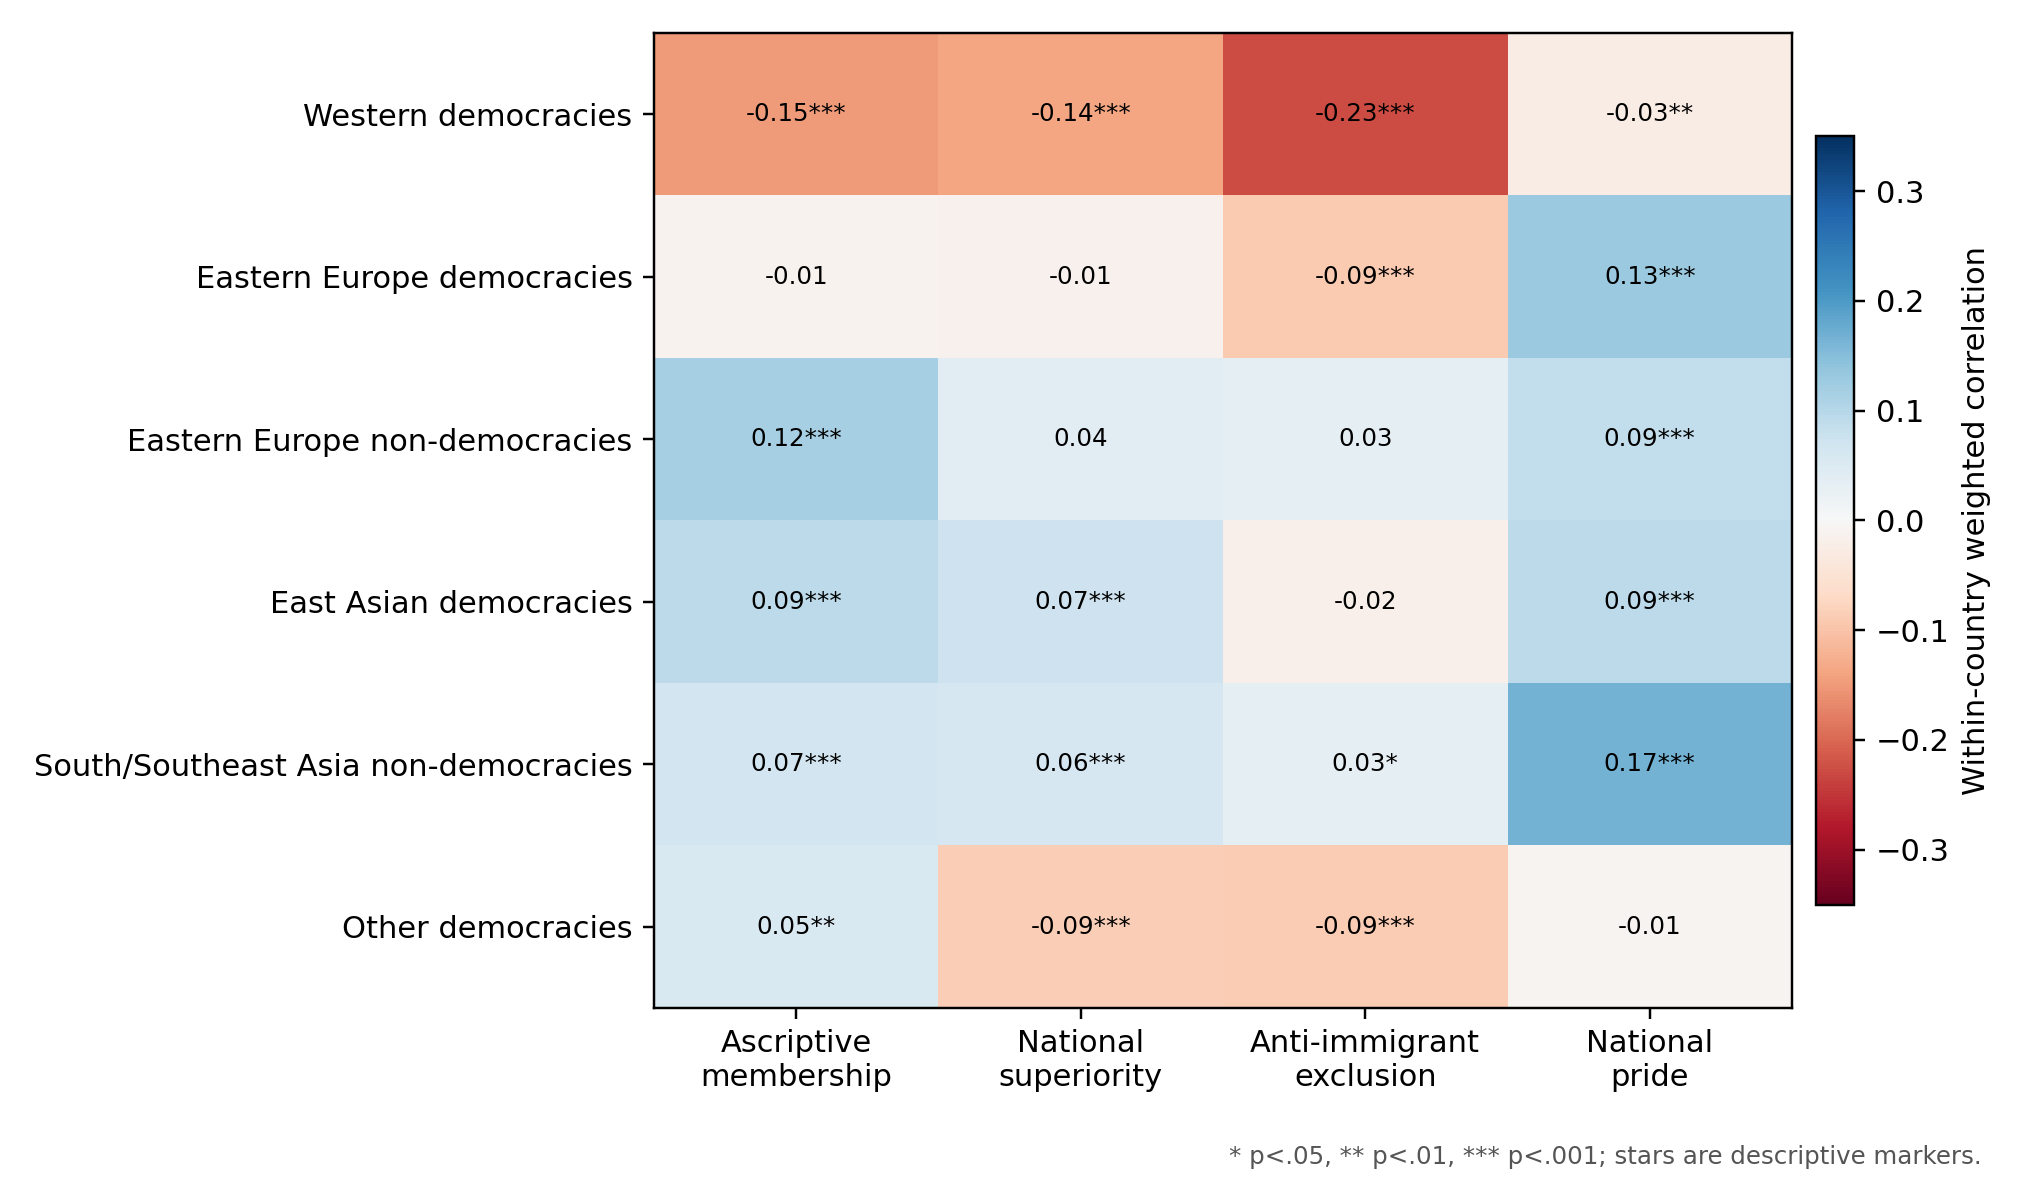
\includegraphics[keepaspectratio,alt={Democratic-rights endorsement and nationalism, by region-regime group (within-country weighted correlations).}]{figures/regional_democratic_rights_heatmap.png}}
\figcap{Democratic-rights endorsement and nationalism, by region-regime group}{Cell entries are within-country weighted correlations (ISSP combined weight, equal country weighting), averaged within each region-regime group. Within Western democracies the rights--exclusion correlations are negative; outside the West they weaken and, in the electoral autocracies, turn positive.}
\end{figure}

\begin{figure}[H]
\centering
\pandocbounded{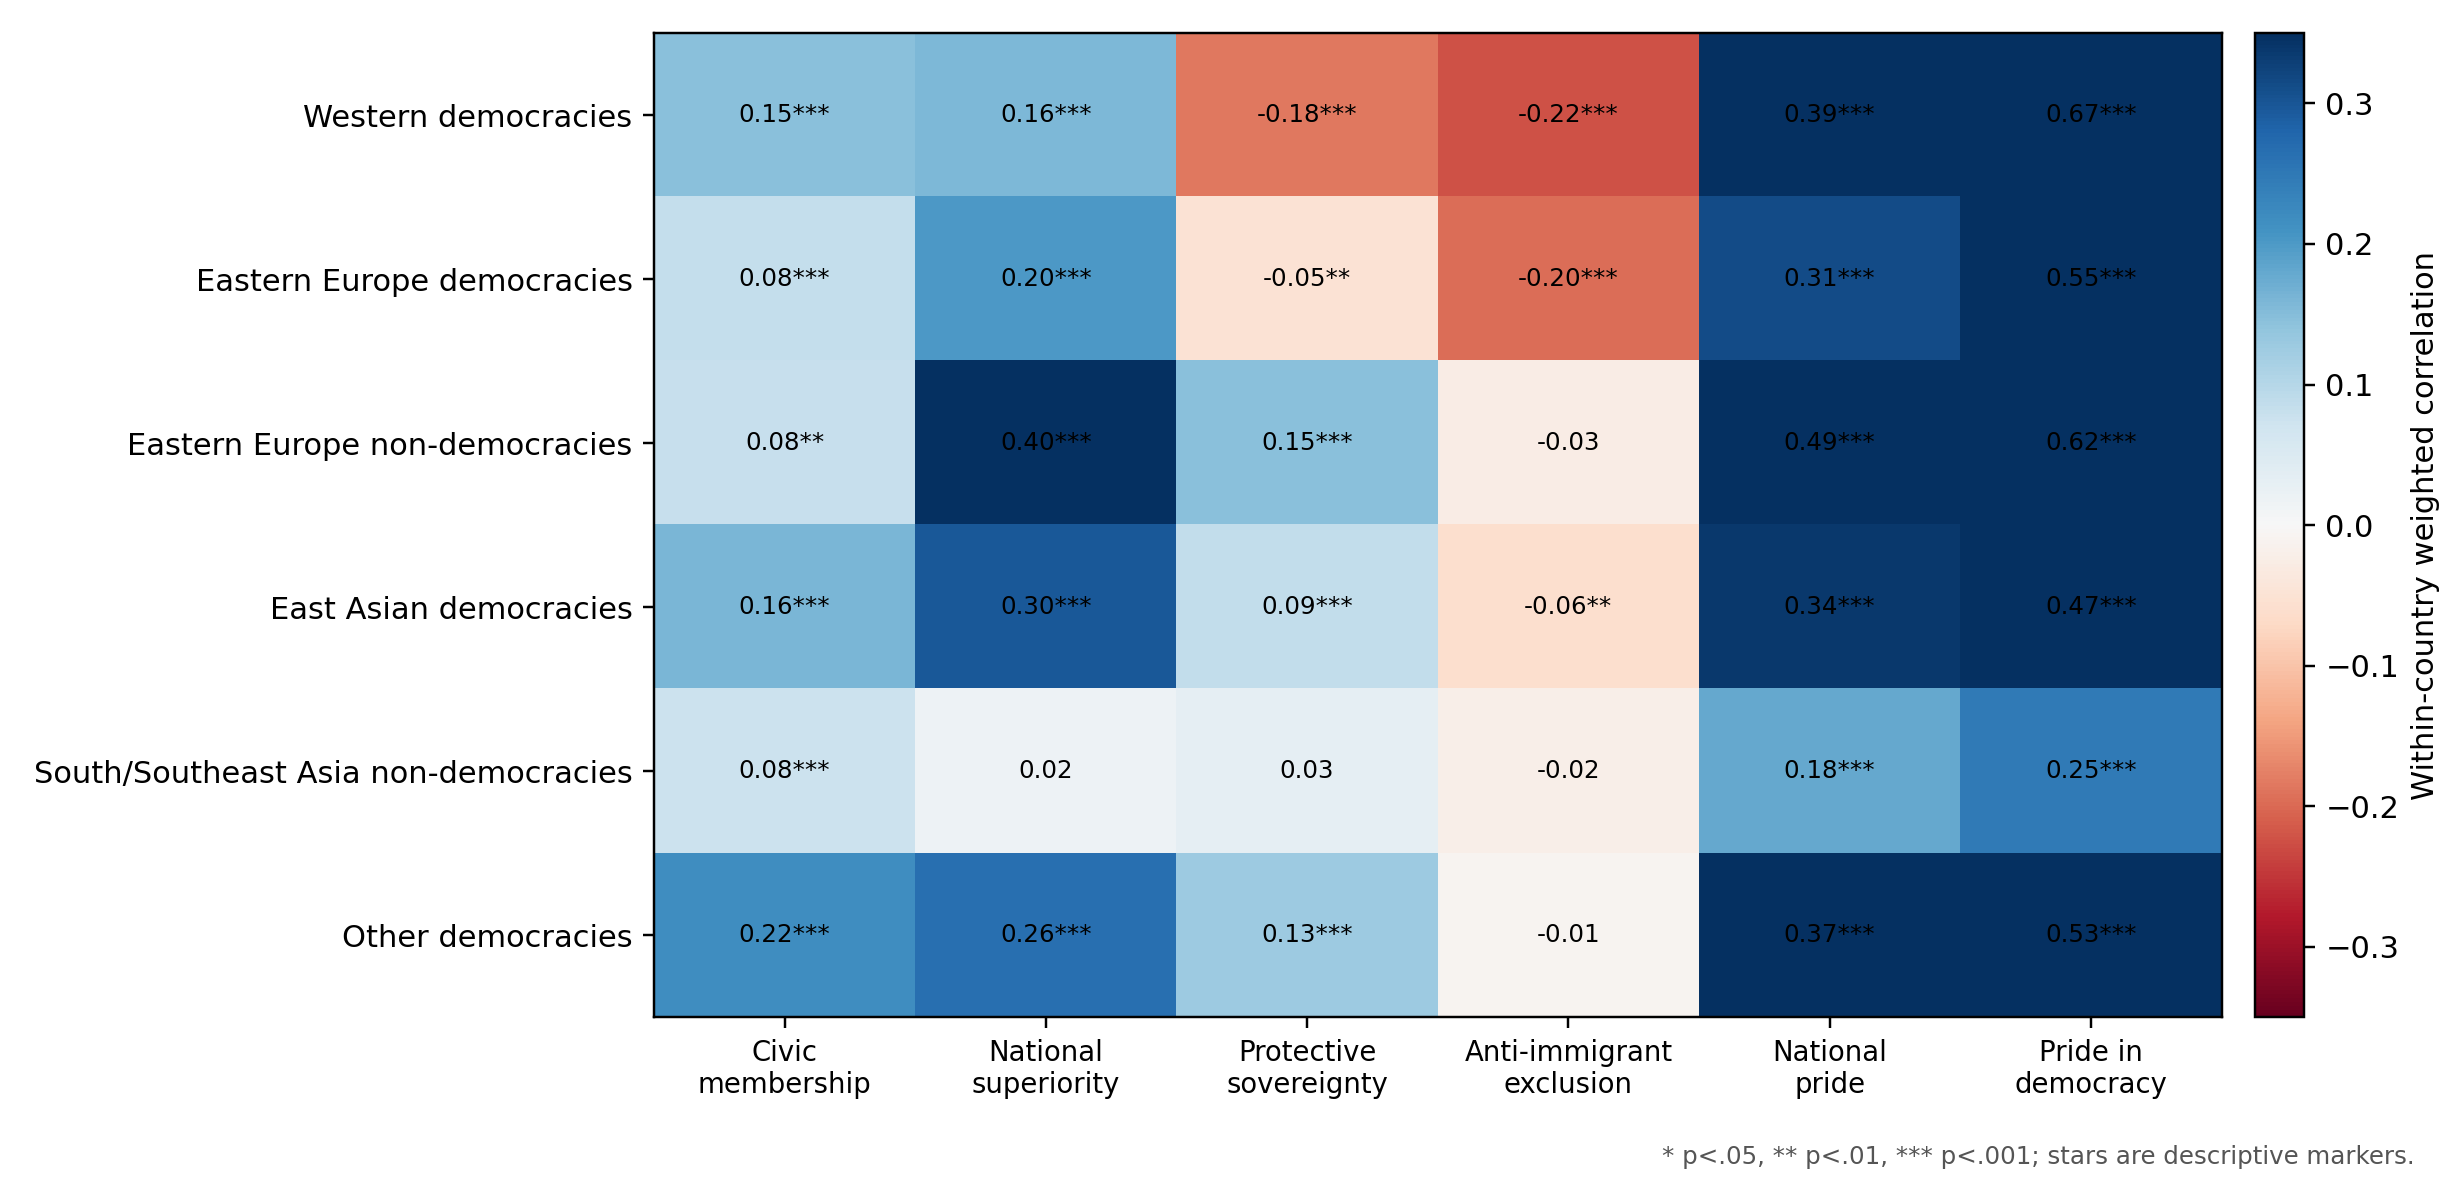
\includegraphics[keepaspectratio,alt={Perceived democratic performance and nationalism, by region-regime group.}]{figures/regional_democracy_performance_heatmap.png}}
\figcap{Perceived democratic performance and nationalism, by region-regime group}{Cell entries are within-country weighted correlations of perceived democratic performance with each nationalism measure, averaged within each region-regime group. Performance tracks pride and superiority across regions, in contrast to the rights pattern above.}
\end{figure}

\clearpage
\section{SI-I. Country-specific adjusted slopes (all outcomes)}\label{si-i.-country-specific-adjusted-slopes-all-outcomes}

\begin{figure}[H]
\centering
\pandocbounded{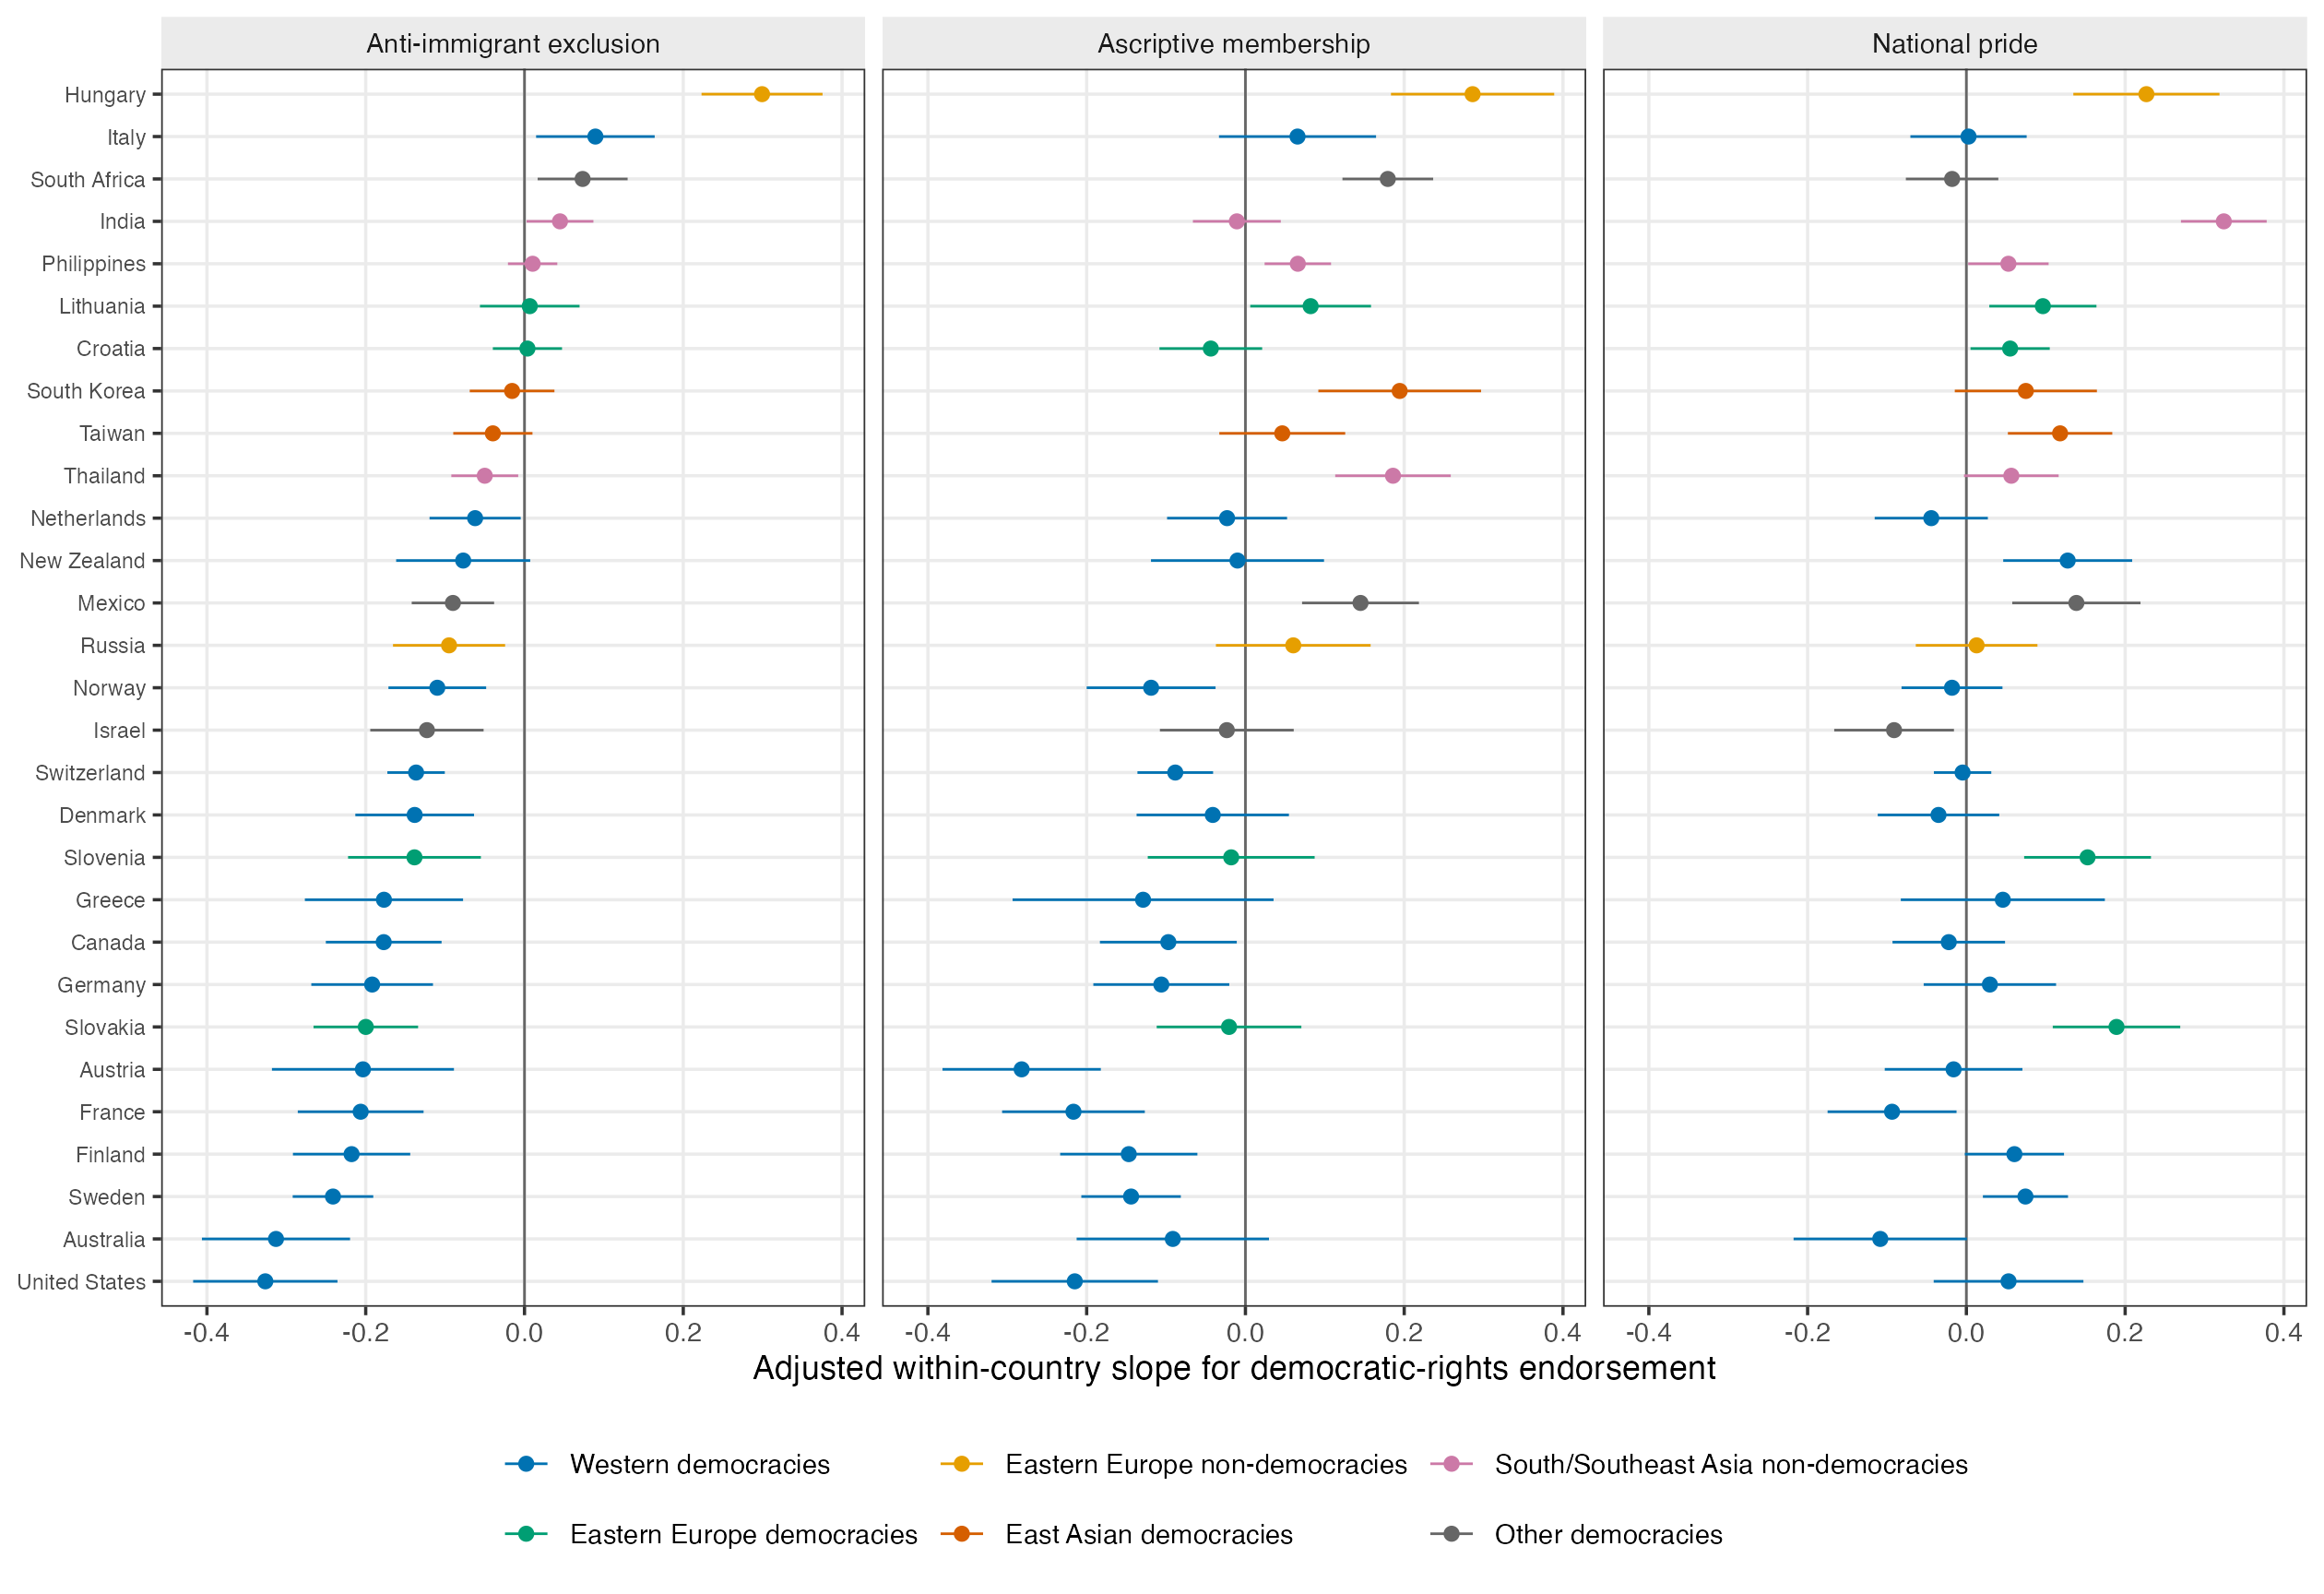
\includegraphics[keepaspectratio,alt={Country-specific adjusted slopes for democratic-rights endorsement (with controls), by outcome.}]{figures/country_adjusted_democratic_rights_slopes.png}}
\figcap{Country-specific adjusted slopes for democratic-rights endorsement, by outcome}{Points are country-specific within-country slopes of each outcome on democratic-rights endorsement, adjusted for individual controls (age, gender, education, left--right placement); bars are 95\% confidence intervals and color denotes region-regime group. Countries share the anti-immigrant ordering of main-text Figure 1. The anti-immigrant panel reproduces that figure; the ascriptive and pride panels extend it to the other outcomes.}
\end{figure}

\section{SI-J. Robustness}\label{si-j.-robustness}

The reversal at the heart of the paper is not an artifact of the regime classification, the choice of index, or the weighting scheme, as five checks confirm.

Design-based weighted estimates agree with the model-based ones. The descriptive within-country correlations (SI-H, computed with \texttt{WEIGHT\_COM} and equal country weighting) agree with the model-based estimates in sign and pattern. The main-text models are unweighted, and design-based weighting does not change the conclusions.

A regime binary reproduces the contrast. Splitting by the simple V-Dem democracy/non-democracy binary, the correlations between democratic-rights endorsement and exclusion are negative within democracies (anti-immigrant −0.18, superiority −0.09, ascriptive −0.08) and positive within the five non-democracies (ascriptive +0.09, superiority +0.05, pride +0.13). The binary is coarse (5 non-democracies) and is reported only as a robustness contrast; the continuous content-of-nationhood moderator is preferred.

An alternative democratic-rights index yields the same pattern. The four-item index, which adds ``adequate standard of living,'' reproduces the result.

The ascriptive outcome carries one caveat. Because the content-of-nationhood moderator is the country mean of ascriptive membership, the moderation of the \emph{ascriptive} slope is partly mechanical, so the main text leads with anti-immigrant exclusion, where moderator and outcome are distinct.

The clustering unit does not matter. Germany and Israel each contribute two ISSP samples (\texttt{c\_sample}); using \texttt{c\_sample} (31 units) rather than country (29) as the grouping factor leaves results unchanged.

\clearpage
\section{SI-K. Descriptive longitudinal panel (1995--2023)}\label{si-k.-descriptive-longitudinal-panel-19952023}

The democratic-rights battery is 2023-only, so the relationship cannot be traced over time. As context, I track the \emph{levels} of two exclusionary-nationalism measures available in all four ISSP National Identity rounds --- ascriptive membership (born + religion importance) and anti-immigrant exclusion (crime, economy, jobs, immigration level) --- for Western versus non-Western countries. This is descriptive and leans on cross-wave comparability, which the invariance results (SI-D) show is imperfect. Country composition also varies by wave, since the 1995 round fields only four Western countries. Read trajectories, not precise levels. The finer region-regime classification used throughout the rest of the analysis is too sparse to follow across waves here, so this panel falls back on a deliberately coarse West / non-West contrast. That split is a convenience of the thin longitudinal data, not a claim that either group is internally uniform or that the two mark a normative or civilizational divide. It is a dispassionate grouping of places by region and regime, and where the better-resolved groups differ in the 2023 cross-section I report those differences directly (SI-B, SI-H).

\begin{figure}[H]
\centering
\pandocbounded{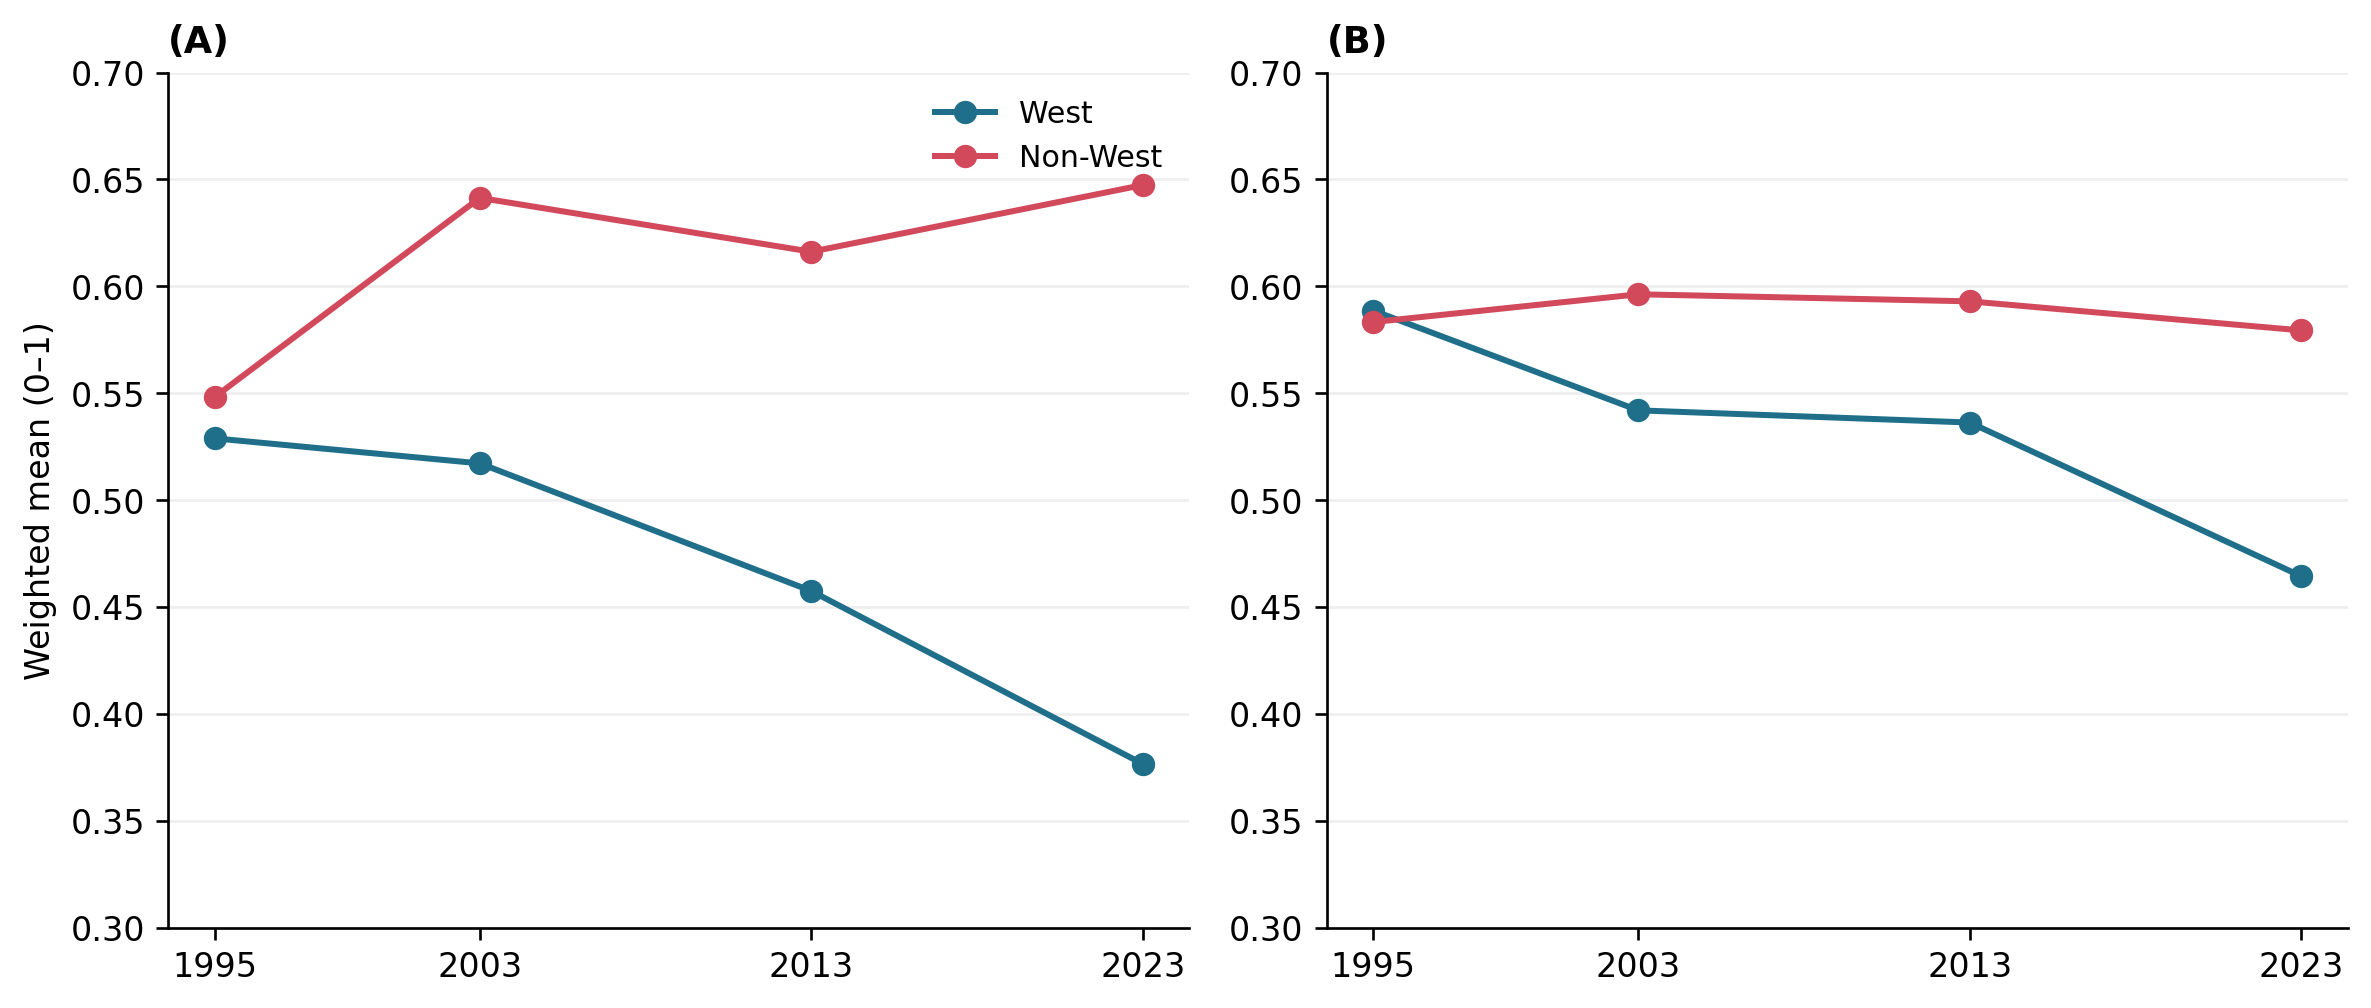
\includegraphics[keepaspectratio,alt={ISSP National Identity 1995--2023. Exclusionary nationalism, West versus non-West (weighted means; composition varies by wave). Panel (A) is the ascriptive (ethnic) conception of nationhood and panel (B) is anti-immigrant exclusion.}]{figures/figS_longitudinal.png}}
\figcap{Exclusionary nationalism, West versus non-West, ISSP National Identity 1995--2023}{Weighted means by wave; panel (A) is the ascriptive (ethnic) conception of nationhood and panel (B) is anti-immigrant exclusion. Country composition varies by wave (1995 includes only four Western countries), and cross-wave comparability is imperfect (SI-D), so read trajectories rather than precise levels. The figure shows a long Western civic turn against flat non-Western levels.}
\end{figure}

{\small\begin{longtable}[]{@{}llrrrr@{}}
\toprule\noalign{}
Measure & Group & 1995 & 2003 & 2013 & 2023 \\
\midrule\noalign{}
\endhead
\bottomrule\noalign{}
\figcap{Exclusionary nationalism by wave, West versus non-West (weighted means)}{Country composition varies by wave; read trajectories, not precise levels.}\\
\endlastfoot
Ascriptive & West & 0.53 & 0.52 & 0.46 & 0.38 \\
& Non-West & 0.55 & 0.64 & 0.62 & 0.65 \\
Anti-immigrant & West & 0.59 & 0.54 & 0.54 & 0.46 \\
& Non-West & 0.58 & 0.60 & 0.59 & 0.58 \\
\end{longtable}}

The descriptive picture is a long Western civic turn: ascriptive and anti-immigrant nationalism have fallen in Western publics since 1995 while remaining flat elsewhere. The civic character of Western nationhood that conditions the 2023 cross-section is thus the product of a multi-decade divergence, not a fixed cultural constant.

\clearpage
\section{SI-L. Democratic socialization in Taiwan and South Korea}\label{si-l-cohort}

Taiwan and South Korea redefined their national projects and democratized recently, Taiwan across the 1990s (with the first direct presidential election in 1996) and South Korea in 1987--1988. Redefining the nation, and the political-cultural change that democratization sets in motion, takes a generation to consolidate rather than all at once. Political identities and orientations crystallize during the formative, ``impressionable'' years and then persist with comparative stability across the life course \citep{mannheim1952generations, jennings1981generations, krosnick1989aging, neundorf2017socialization}, so a cohort that comes of age under one national-institutional settlement tends to carry its imprint forward. I bracket that formative window as ages 12--25, running from the onset of political awareness through early adulthood, and ask whether citizens whose entire window fell under democratic institutions hold more civic, less ascriptive conceptions of nationhood. A respondent is classified as democratically socialized if they reached age 12 at or after the transition, so that the whole 12--25 window post-dates it (born in or after 1984 in Taiwan, 1975 in South Korea). Cell entries are weighted means. Ascriptive membership and anti-immigrant exclusion run from 0 to 1 with higher values more exclusionary, and the civic-minus-ethnic column is the civic-membership advantage over ascriptive membership, where higher is more civic.

\begin{table}[H]
\centering
\small
\begin{tabular}{llrrrr}
\toprule
Country & Cohort & $N$ & Ascriptive & Civic $-$ ethnic & Anti-immigrant \\
\midrule
Taiwan & Democratically socialized & 426 & 0.33 & $+0.49$ & 0.39 \\
Taiwan & Earlier cohort & 1{,}137 & 0.46 & $+0.41$ & 0.47 \\
South Korea & Democratically socialized & 491 & 0.55 & $+0.18$ & 0.55 \\
South Korea & Earlier cohort & 739 & 0.61 & $+0.16$ & 0.55 \\
\bottomrule
\end{tabular}
\figcap{Conceptions of nationhood by democratic-socialization cohort, Taiwan and South Korea}{Cell entries are weighted means. ``Democratically socialized'' respondents reached age 12 at or after the transition (born in or after 1984 in Taiwan, 1975 in South Korea). Ascriptive membership and anti-immigrant exclusion run 0--1 with higher values more exclusionary; the civic-minus-ethnic column is the civic-membership advantage over ascriptive membership, where higher is more civic. The civic gradient is more than twice as steep in Taiwan.}
\end{table}

The pattern matches the expectation. In Taiwan the democratically socialized cohort is markedly more civic. Its mean endorsement of ascriptive membership (0.33) sits 0.13 below the earlier cohort (0.46) and reaches the Western level, where the mean is about 0.36 (SI-B). In South Korea the same comparison yields a much smaller gap (0.55 against 0.61), and even the younger cohort remains strongly ethnic in its conception of nationhood, well above the Western level. The generational gradient in the civic conception of nationhood is more than twice as steep in Taiwan as in South Korea. This comparison is observational and confounds cohort with life cycle, so it is suggestive rather than decisive. Comparing the cohort gap across the two cases nonetheless follows the design-based logic for separating cohort from life-cycle effects \citep{dinas2014ageperiodcohort}. A universal age effect would not produce a Taiwan gradient twice the Korean one, nor would it bring Taiwan's young cohort to Western civic levels. The pattern instead fits Taiwan's more thorough post-1990s shift toward a civic, territorial conception of the nation. This convergence bears on how the cross-section should be read. The civic character of Western nationhood is itself a recent, multi-decade development (SI-K), and Taiwan's democratically socialized cohort has reached a comparably civic conception within a single generation. The difference between civic and ethnic conceptions of nationhood is therefore one of historical and institutional trajectory rather than of fixed East/West essence. Taiwan's youngest citizens are the clearest case of an ethnically defined nation reaching a civic conception within a generation.

The reorientation shows up not only in the level of ascriptive nationhood but in the democratic-rights relationship itself. The table below reports the within-cohort correlation of democratic-rights endorsement with anti-immigrant exclusion and with ascriptive membership.

\begin{table}[H]
\centering
\small
\begin{tabular}{llrr}
\toprule
Country & Cohort & $r$(rights, anti-immigrant) & $r$(rights, ascriptive) \\
\midrule
Taiwan & Democratically socialized & $-0.10$ & $-0.01$ \\
Taiwan & Earlier cohort & $+0.02$ & $+0.10$ \\
South Korea & Democratically socialized & $+0.02$ & $+0.14$ \\
South Korea & Earlier cohort & $-0.04$ & $+0.14$ \\
\bottomrule
\end{tabular}
\figcap{Within-cohort correlation of democratic-rights endorsement with exclusion, Taiwan and South Korea}{Cell entries are within-cohort correlations of democratic-rights endorsement with anti-immigrant exclusion and with ascriptive membership, without controls. The Taiwanese democratically socialized cohort displays the Western, restraining pattern; the South Korean cohorts do not shift. Read as suggestive.}
\end{table}

In Taiwan the democratically socialized cohort displays the Western, restraining pattern. Democratic-rights endorsement is negatively correlated with anti-immigrant exclusion ($-0.10$) and unrelated to ascriptive membership ($-0.01$), whereas among the earlier cohort the same correlations are flat or positive ($+0.02$ and $+0.10$). In South Korea the relationship does not shift across cohorts. Democratic-rights endorsement remains positively associated with ascriptive nationhood in both the young and the old ($+0.14$), consistent with an ethnic conception that has not reoriented. These are subgroup correlations without controls and should be read as suggestive, but they show the paper's central moderation playing out within a single country over time.

\clearpage
\section{SI-M. Reproducibility}\label{si-m.-reproducibility}

The replication package holds the analysis scripts in \texttt{code/} and writes all derived tables and figures to \texttt{outputs/}. The scripts are:

\begin{itemize}
\tightlist
\item
  \texttt{issp2023\_democracy\_nationalism.py} --- descriptive measures, regional correlations, heatmaps.
\item
  \texttt{vdem\_extract.R} --- V-Dem v15 indices for the 29 countries.
\item
  \texttt{build\_analysis\_data.py} --- assembles the analysis-ready individual file and country-level moderators (using the V-Dem indices above).
\item
  \texttt{measurement\_invariance.R} --- multi-group CFA and alignment (lavaan, semTools, sirt).
\item
  \texttt{multilevel\_models.R} --- random-slope models and cross-level interactions (lme4).
\item
  \texttt{diagnostic\_secondstage.R} --- country-level second-stage regressions.
\item
  \texttt{longitudinal\_trends.py} --- 1995--2023 harmonization.
\item
  \texttt{cohort\_test.py} --- democratic-socialization cohort test (SI-L).
\item
  \texttt{figures\_v2.py} and \texttt{figures\_ggrepel.R} --- publication figures (the latter, in ggplot2 with ggrepel, produces the two country-level figures and the supplementary slopes figure).
\end{itemize}

The driver \texttt{master.sh} runs these scripts in dependency order and writes all derived outputs to \texttt{outputs/}; the manuscript PDFs are then built with \texttt{make} in the manuscript source directory. \texttt{README.md} gives the figure/table-to-script crosswalk.

\subsection*{Data access}

The ISSP 2023 microdata (\texttt{ZA10010}) are obtained free from the GESIS Data Archive after registration and are not redistributed here, and the earlier waves (\texttt{ZA2880}, \texttt{ZA3910}, \texttt{ZA5950}) are obtained the same way. V-Dem v15 is retrieved through the \texttt{vdemdata} R package, installed with \texttt{remotes::\allowbreak install\_github(\allowbreak"vdeminstitute/\allowbreak vdemdata")}.

\subsection*{Software}

The pipeline uses Python 3 (pandas, numpy, pyreadstat, scipy, matplotlib) and R 4.5 (lavaan, semTools, sirt, lme4, ggplot2, ggrepel, vdemdata), with pandoc and pdflatex for the manuscript. It is deterministic except for \texttt{sirt::invariance.alignment} (SI-D), whose optimizer is seeded for exact reproduction.
